% !TEX TS-program = pdfLaTeX+shellescape
% !TEX encoding = UTF-8 Unicode

\documentclass[class=beamer,tikz]{standalone}
\setbeamertemplate{navigation symbols}{} % For delete the navigation symbols
\usefonttheme{professionalfonts}
\usepackage{luatexja}
% \usepackage{pgfplots}
% \pgfplotsset{compat=1.17}

\usepackage{colortbl,array,xcolor}
\usepackage{amsmath,amsfonts}

\begin{document}
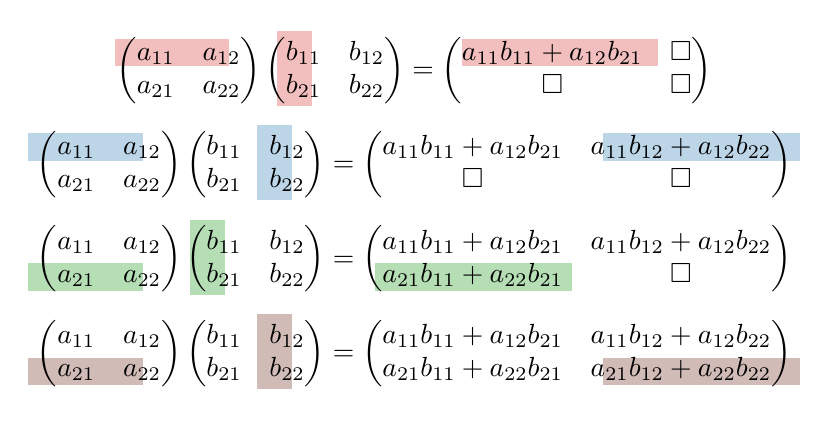
\begin{tikzpicture}
    \definecolor{tab_red}{HTML}{d62728}
    \definecolor{tab_blue}{HTML}{1f77b4}
    \definecolor{tab_green}{HTML}{2ca02c}
    \definecolor{tab_yellow}{HTML}{8c564b}
    %\draw[help lines] (0,0) grid (12,10);
    \path[fill=tab_red!30] (2.20,4.65) rectangle (3.65,5.00);
    \path[fill=tab_red!30] (4.25,4.15) rectangle (4.70,5.10);
    \path[fill=tab_red!30] (6.60,4.65) rectangle (9.10,5.00);
    \path[fill=tab_blue!30] (1.10,3.45) rectangle (2.55,3.80);
    \path[fill=tab_blue!30] (4.00,2.95) rectangle (4.45,3.90);
    \path[fill=tab_blue!30] (8.40,3.45) rectangle (10.90,3.80);
    \path[fill=tab_green!35] (1.10,1.80) rectangle (2.55,2.15);
    \path[fill=tab_green!35] (3.15,1.75) rectangle (3.60,2.70);
    \path[fill=tab_green!35] (5.50,1.80) rectangle (8.00,2.15);
    \path[fill=tab_yellow!40] (1.10,0.60) rectangle (2.55,0.95);
    \path[fill=tab_yellow!40] (4.00,0.55) rectangle (4.45,1.50);
    \path[fill=tab_yellow!40] (8.40,0.60) rectangle (10.90,0.95);
    
    \node (matrix0) at (6.0,4.6) {
        $\begin{pmatrix}
            a_{11} & a_{12} \cr
            a_{21} & a_{22} 
        \end{pmatrix}\begin{pmatrix}
            b_{11} & b_{12} \cr 
            b_{21} & b_{22}
        \end{pmatrix} = \begin{pmatrix}
            a_{11}b_{11}+a_{12}b_{21} & \square \cr 
            \square & \square 
        \end{pmatrix}$
    };
    \node (matrix1) at (6.0,3.4) {
        $\begin{pmatrix}
            a_{11} & a_{12} \cr
            a_{21} & a_{22} 
        \end{pmatrix}\begin{pmatrix}
            b_{11} & b_{12} \cr 
            b_{21} & b_{22}
        \end{pmatrix} = \begin{pmatrix}
            a_{11}b_{11}+a_{12}b_{21} & a_{11}b_{12}+a_{12}b_{22} \cr 
            \square & \square 
        \end{pmatrix}$
    };
    \node (matrix2) at (6.0,2.2) {
        $\begin{pmatrix}
            a_{11} & a_{12} \cr
            a_{21} & a_{22} 
        \end{pmatrix}\begin{pmatrix}
            b_{11} & b_{12} \cr 
            b_{21} & b_{22}
        \end{pmatrix} = \begin{pmatrix}
            a_{11}b_{11}+a_{12}b_{21} & a_{11}b_{12}+a_{12}b_{22} \cr 
            a_{21}b_{11}+a_{22}b_{21} & \square 
        \end{pmatrix}$
    };
    \node (matrix3) at (6.0,1) {
        $\begin{pmatrix}
            a_{11} & a_{12} \cr
            a_{21} & a_{22} 
        \end{pmatrix}\begin{pmatrix}
            b_{11} & b_{12} \cr 
            b_{21} & b_{22}
        \end{pmatrix} = \begin{pmatrix}
            a_{11}b_{11}+a_{12}b_{21} & a_{11}b_{12}+a_{12}b_{22} \cr 
            a_{21}b_{11}+a_{22}b_{21} & a_{21}b_{12}+a_{22}b_{22}
        \end{pmatrix}$
    };
\end{tikzpicture}
\end{document}